\chapter{Künstliche Intelligenz}
\label{chap:ai}

In diesem Kapitel wird die KI erklärt.

\section{Was ist KI?}

Künstliche Intelligenz ist ein Teilgebiet der Informatik, das sich mit der Entwicklung von Computersystemen befasst, die Aufgaben erfüllen können, die normalerweise menschliche Intelligenz erfordern. \textit{"KI wird weltweit für verschiedene militärische Aufgaben eingesetzt, um Prozesse zu optimieren und zu beschleunigen." \citep{ethics-ai-wikipedia}}\newline
KI existiert schon länger, jedoch war sie nicht so fortgeschritten wie heute. Vor ChatGPT gab keinen KI, welche in der Lage war Fragen und Text zu analysieren und auf diese Antworten zu geben. Dank Nvidia, ein Frima welche GPUs(Graphical Processing Unit) herstellt. Konnte OpenAI ChatGPT entwickeln.

\section{Wie analysiert KI Texte?}

KI analysiert Texte, indem sie Algorithmen nutzt, um aus riesigen Datensätzen Regeln abzuleiten oder Muster zu erkennen. Dies ermöglicht es, Verhaltensmuster oder -abweichungen zu erkennen, die die Grundlage für automatisierte Entscheidungen bilden. \textit{"Die Interpretation menschlicher Sprache durch Maschinen besitzt bei der KI-Forschung eine entscheidende Rolle. So ergeben sich etwaige Ergebnisse des Turing-Tests vor allem in Dialogsituationen, die bewältigt werden müssen." \citep{ai-wikipedia}}

\section{Vor- und Nachteile von KI}

Vorteile der KI sind eine hohe Reaktionsgeschwindigkeit und Genauigkeit, die Möglichkeit, große Informationsmengen schnell zu verarbeiten, die Reduzierung der menschlichen Kosten des Krieges und die Chance, Probleme zu lösen, die für Menschen aufgrund ihrer limitierten Kapazitäten schwer zu lösen sind. Nachteile der KI könnten sein, dass KI-Maschinen sich gegen die Interessen der Menschen wenden könnten und dass KI diskriminierend sein oder Vorurteile verstärken könnte. Es ist wichtig, dass der Einsatz von KI ethischen Grundsätzen folgt und die Würde des Menschen sowie Grundrechte respektiert.\newline
Die Nachteile der KI sind hauptsächlich diese rechnen mit Daten. \textit{"von Handlungen und Entscheidungen, die durch automatisierte/künstliche Intelligenz (KI) in Bezug auf Daten im Allgemeinen und personenbezogene Daten im Besonderen gesteuert werden" \citep{ethics-cognizant}} Obwohl die KI effizienter ist, kann sie nicht selber nachdenken. Ebenfalls hat die KI nicht so viel Speicherplatz für ihre Datenback, wie es Menschen haben. Für uns Menschen ist das Gehirn eine Art riesige Datenbank auf die wir zurückgreifen können.\newline
KI kann oft falsch liegen, weil Algorithmen für KI und maschinelles Lernen aus den Rückmeldungen der Nutzer lernen, basierend auf Trainingsdaten, die Verzerrungen enthalten können, wenn bestimmten Merkmalen und Eigenschaften der Vorzug gegeben wird. Dies kann zu Fehlern oder Lücken im Training führen, die dazu führen können, dass der KI falsches Verhalten beigebracht wird, das nicht mit menschlichen Werten vereinbar ist.

\begin{figure}[h]
    \centering
    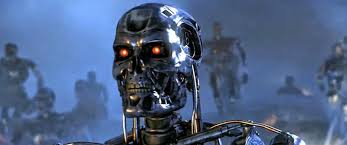
\includegraphics[width=0.5\textwidth]{rogue_ai.jpeg}
    \caption{Eine fiktionales Beispiel einer schlechten KI}
    \label{fig:rogueAI}
\end{figure}
